\chapter{Implementación}
\label{cha:Implementation}

En este capítulo se abordará los aspectos de implementación de SheetChat, que es un software que permite interpretar el DSL definido en el Capítulo \ref{cha:AnalysisAndDesign} y desplegar un chatbot sobre la plataforma Slack.

Para abordar los aspectos de implementación, el capítulo se dividirá en tres secciones o apartados principales. En el Apartado \ref{sec:Botkit} se presentará la plataforma de desarrollo de bots utilizada, Botkit, desarrollada en Javascript. En el Apartado \ref{sec:ImplementationLanguage} se hablará del lenguaje de programación utilizado y del ecosistema utilizado. Por último, en el Apartado \ref{sec:AlaSQL} se hablará del motor SQL utilizado para permitir al DSL el uso de consultas enriquecidas con funciones matemáticas que se ha comentado en el Apartado \ref{sec:Queries}.

Como se puede observar en la Figura \ref{fig:UMLComponents}, se han utilizado otros servicios web para que forman parte del funcionamiento de SheetChat, pero de los que no se hablará en este capítulo. Estos son Wit.ai\footnote{Sitio web de Wit.ai: \url{https://wit.ai}} y la API de Google Spreadsheets\footnote{Sitio web de la documentación de la API de Google SpreadSheet: \url{https://developers.google.com/sheets/}}. Wit.ai se utiliza en la desambiguación de intents y reconocimiento de entidades, explicado en el Apartado \ref{sec:Chat}. Sobre Wit.ai se puede profundizar en el Anexo \ref{anx:witai}. La API de Google Spreadsheets permite la obtención de los datos de forma matricial de la hoja de cálculo alojada en Google Docs.

\begin{figure}[htb]
	\centering
	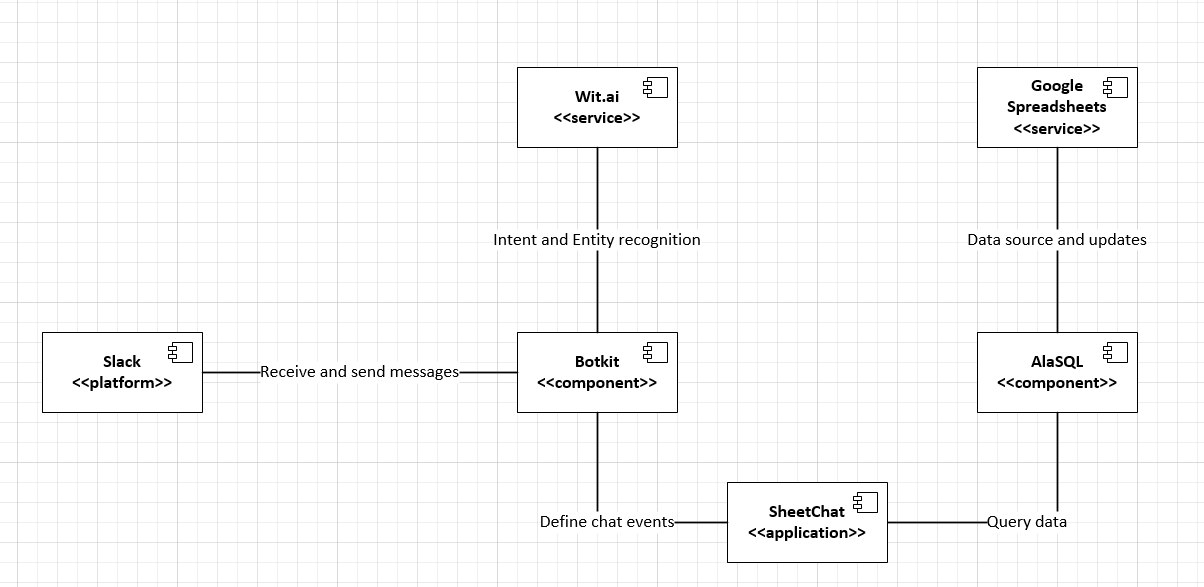
\includegraphics[width=0.8\textwidth]{./figs/UMLComponents.png}
	\caption{Diagrama de componentes UML de SheetChat.}
	\label{fig:BotkitConversation}
\end{figure}

Cabe destacar que el código fuente y los ejemplos del Capítulo \ref{cha:CaseStudies} están accesibles en el siguiente repositorio de Github: \url{https://github.com/haritzmedina/Sheetbot}.


\section{Botkit}
\label{sec:Botkit}

Botkit, es una librería que permite la programación de manera más sencilla de Chatbots distribuida bajo licencia MIT. Al igual que otras plataformas mencionadas en el Apartado \ref{sec:PlataformasChatbot}, como Microsoft Bot Framework o la API de bots de Telegram, Botkit permite la abstracción de algunos aspectos de programación. Botkit es una librería desarrollada por Howdy.ai. Está programada en Javascript y funciona sobre Node.js \footnote{Node.js, es un entorno de ejecución de Javascript multi-plataforma: \url{https://nodejs.org/en/}}.

Botkit permite desarrollar bots para Slack, Facebook Messenger y Twilio. Como se ha mencionado previamente, en este trabajo se ha focalizado su uso sobre Slack. Para su uso simplemente será necesario crear un nuevo bot en Slack (o como se llama en Slack, una App \footnote{Creación de apps o bots en Slack: \url{https://api.slack.com/bot-users}}) e indicarle el token de acceso al bot.

Botkit presenta un sistema relativamente sencillo para crear bots conversacionales. Se basa en una programación orientada a eventos, de ahí que case perfectamente con Javascript, que es un lenguaje dirigido por eventos. Los tipos de eventos que se pueden definir son los siguientes:
\begin{itemize}
	\item \textbf{Escuchar mensajes}: se puede establecer que Botkit esté a la escucha de un mensaje concreto y asociar una funcionalidad en caso de que se reciba el mensaje que se desea recibir. Se puede establecer en qué canales se desea escuchar dependiendo de la plataforma. En Slack los canales son: mensaje privado, mención a él en un grupo (donde esté añadido como miembro el bot) o mensaje recibido por cualquier canal.
	\item \textbf{Responder/Enviar mensajes}: una funcionalidad habitual cuando se recibe un mensaje es contestar con otro. En slack se puede definir un mensaje de respuesta más o menos elaborado, con emoticonos, textos coloreados, etc.
\end{itemize}

Botkit además de gestionar recepción y envíos de mensajes es capaz de entablar conversaciones. De esta manera se puede mantener la información intercambiada durante la conversación ya que puede ser relevante para dar una respuesta más precisa. En la Figura \ref{fig:BotkitConversation} se puede observar un ejemplo de conversación. En este caso el usuario ha pedido una pizza y el bot le va preguntando por el tipo de pizza, el tamaño y dónde debe de entregarse. Estos tres datos van asociados al mismo pedido, por lo que puede ser interesante utilizar la noción de conversación que Botkit proporciona.

\begin{figure}[htb]
	\centering
	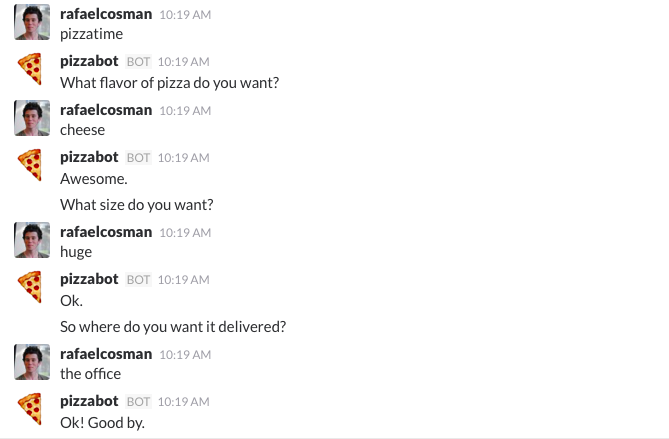
\includegraphics[width=0.8\textwidth]{./figs/BotkitConversation.png}
	\caption{Una conversación con Botkit sobre Slack.}
	\label{fig:BotkitConversation}
\end{figure}

En la generación de bots mediante SheetChat se ha utilizado esta característica de entablar conversación también. La creación de una conversación permite ir recabando las entidades necesarias para hacer el filtrado sobre los datos de la tabla y proporcionar el resultado que el usuario necesita. De igual manera, Botkit proporciona mecanismos de repetición de preguntas para el caso de que no haya podido interpretar la información que el usuario le ha proporcionado.

Como se ha mencionado previamente, en Botkit el funcionamiento reside en que necesita escuchar un mensaje para poder comunicar algo. Para poder decidir si la conversación que hay que abrir pertenece a un Intent o a otro se ha utilizado la técnica de \emph{Intent Disambiguation} (ver Apartado \ref{sec:Chat}) mediante la herramienta de procesamiento del lenguaje natural Wit.ai. Para aunar el uso de Botkit con el de Wit.ai existe un middleware que se ha tenido que adaptar para este trabajo llamado \href{https://github.com/haritzmedina/botkit-middleware-witai}{botkit-middleware-witai}.

\section{Lenguaje de implementación}
\label{sec:ImplementationLanguage}

El lenguaje de implementación utilizado es Javascript. En gran medida impuesto por la librería en la que se apoya SheetChat y que se acaba de exponer, Botkit, pero también porque es un lenguaje adecuado para el desarrollo de agentes conversacionales. En particular se ha utilizado el estándar ECMAScript2015\footnote{Sitio web de ECMAScript2015: \url{http://www.ecma-international.org/ecma-262/6.0/}} o ECMA 6, que viene a ser la nueva versión de Javascript.

Tal y como se ha mencionado antes, el desarrollo se ha realizado sobre Node.js. Cabe destacar que los bots se ejecutan de manera local y se conectan a las diferentes APIs de los servicios de mensajería instantánea, como puede ser en este caso Slack. La idea es que esta aplicación resida en un servidor dedicado que permita su ejecución dando disponibilidad al bot de manera continua.

\section{Motor SQL para consultas. AlaSQL}
\label{sec:AlaSQL}

Una de las piezas fundamentales y sobre las que se basa la teoría de este proyecto son las hojas de cálculo y las consultas y filtrados que se le pueden realizar. Google SpreadSheet dentro de su API no proporciona filtrados de ningún tipo, ni un lenguaje potente para realizar consultas específicas sobre los datos. Es por ello que se ha decidido utilizar una implementación de SQL para javascript, llamada AlaSQL \footnote{AlaSQL, una implementación de base de datos SQL en memoria en javascript: \url{http://alasql.org/}}.

El método de trabajo con AlaSQL en SheetChat es sencillo. Las filas y columnas que se reciben de Google SpreadSheet se traducen a tablas relacionales, cada tabla está representada por los valores de una hoja de cálculo. En caso de que los datos se actualicen, estos serán actualizados en la tabla de la base de datos en memoria de AlaSQL.

AlaSQL permite el almacenamiento en ficheros, importar datos de CSV, etc. Aunque en este caso sólo se ha utilizado el almacenamiento en memoria de los datos de las hojas de cálculo. Esto reduce en gran medida el tamaño de los datos que un Chatbot puede tener, pero resulta suficiente para un Chatbot de auto-consumo, y la velocidad de consulta es mucho mayor.

Cuando un usuario realiza una petición de unos datos al chatbot, estas consultas se traducen a sentencias SQL que serán ejecutadas sobre AlaSQL. Basándonos en el modelo de características de la Figura \ref{fig:FeatureModel}, se utiliza el response para definir las columnas a mostrar, la hoja de cálculo del intent como la tabla de la base de datos y las entidades cómo filtros. Suponiendo que la respuesta que da el Chatbot es ``Examen1, Examen2, Examen3'', la hoja de cálculo es ``Notas'' y la entidad requerida es ``Alumno'', la consulta se traduciría a algo similar a esta sentencia SQL: \emph{SELECT Examen1, Examen2, Examen3 FROM Notas WHERE Alumno='X'}.

De esta manera se pueden realizar consultas más elaboradas, con funciones tipicas de SQL como SUM, AVG, MAX, LIKE,... siempre que se mantenga la estructura de la consulta. Se descartó la idea de permitir al usuario que pudiese definir sus propias sentencias SQL limitándolas a la estructura SELECT-FROM-WHERE por las siguientes razones:
\begin{itemize}
	\item La idea, de cara al futuro, es poder generar la sintaxis concreta de SheetChat mediante una herramienta gráfica que haga mucho más sencilla la especificación de los bots y no tenga el usuario que aprender el DSL.
	\item La idea no es consultar datos que requieran un procesamiento muy complejo, ya que para el procesamiento de fórmulas matemáticas complejas ya está la propia hoja de cálculo. El objetivo es poder prestar unas entidades derivadas de manera sencilla.
\end{itemize}